\documentclass[10pt,a4paper]{article}
\usepackage[a4paper, margin=2.0cm]{geometry}
\usepackage{fontspec}
\usepackage{xcolor}
\usepackage{titlesec}
\usepackage{fancyhdr}
\usepackage{booktabs}
\usepackage{enumitem}
\usepackage{amsmath}
\usepackage{tcolorbox}
\usepackage{graphicx}
\usepackage{tikz}
\usepackage[colorlinks=true, linkcolor=chulapink, urlcolor=chulapink, citecolor=chulapink]{hyperref}

% TikZ Libraries
\usetikzlibrary{shapes.geometric, arrows.meta, positioning, calc}

% Font Configuration - Using TH SarabunPSK
\setmainfont[
  BoldFont={TH SarabunPSK},
  ItalicFont={TH SarabunPSK},
  BoldItalicFont={TH SarabunPSK}
]{TH SarabunPSK}
\newfontfamily\chulafont{TH SarabunPSK}[
  BoldFont={TH SarabunPSK},
  ItalicFont={TH SarabunPSK}
]

% Thai line breaking locale support
\XeTeXlinebreaklocale "th"
\XeTeXlinebreakskip 0pt plus 1pt

% Custom Color Definitions for Badges
\definecolor{chulapink}{HTML}{B81D67}
\definecolor{darkblue}{HTML}{1A365D}
\definecolor{charcoal}{HTML}{2D3748}
\definecolor{lightgray}{HTML}{F7FAFC}
\definecolor{bordergray}{HTML}{E2E8F0}

\definecolor{badgen8n}{HTML}{FF2E00}
\definecolor{badgeSheets}{HTML}{0F9D58}
\definecolor{badgeGemini}{HTML}{8E7CC3}
\definecolor{badgeMeta}{HTML}{0668E1}
\definecolor{badgeTikTok}{HTML}{000000}
\definecolor{badgePlaywright}{HTML}{2E8B57}
\definecolor{badgeApify}{HTML}{FF6B6B}
\definecolor{badgeSupabase}{HTML}{3ECF8E}
\definecolor{badgePowerBI}{HTML}{F2C811}
\definecolor{badgeLINE}{HTML}{06C755}
\definecolor{badgeDiscord}{HTML}{5865F2}

% Badge Macro representing tool logos
\newcommand{\logobadge}[2]{%
  \begin{tikzpicture}[baseline=(char.base)]
    \node[draw=badge#1, fill=badge#1!10, rounded corners=3pt, inner sep=2pt, font=\scriptsize\bfseries, text=badge#1, minimum height=0.4cm] (char) {#2};
  \end{tikzpicture}%
}

% Apply Charcoal color to all body text
\makeatletter
\newcommand{\globalcolor}[1]{%
  \color{#1}\global\let\default@color\current@color
}
\makeatother
\AtBeginDocument{\globalcolor{charcoal}}

% Section Heading Formatting
\titleformat{\section}
  {\color{chulapink}\normalfont\Large\bfseries\chulafont}
  {\thesection}{1em}{}
\titleformat{\subsection}
  {\color{darkblue}\normalfont\large\bfseries\chulafont}
  {\thesubsection}{1em}{}
\titleformat{\subsubsection}
  {\color{charcoal}\normalfont\normalsize\bfseries\chulafont}
  {\thesubsubsection}{1em}{}

\titlespacing*{\section}{0pt}{1.2ex plus 1ex minus .2ex}{0.6ex plus .2ex}
\titlespacing*{\subsection}{0pt}{1.0ex plus 1ex minus .2ex}{0.5ex plus .2ex}

% Header and Footer Setup
\pagestyle{fancy}
\fancyhf{}
\fancyhead[L]{\chulafont\small\color{chulapink} Chula Tech Startup 2026}
\fancyhead[R]{\chulafont\small\color{charcoal} เอกสารประกอบการสมัครฝ่าย Innovation}
\fancyfoot[C]{\thepage}
\renewcommand{\headrulewidth}{0.4pt}
\renewcommand{\footrulewidth}{0.4pt}

% Callout Box Styling
\newtcolorbox{highlightbox}{
  colback=chulapink!3,
  colframe=chulapink!40,
  arc=4pt,
  boxrule=0.8pt,
  left=12pt,
  right=12pt,
  top=8pt,
  bottom=8pt
}

\begin{document}

% Title Page / Header Block
\begin{center}
  \vspace*{0.3cm}
  {\Huge\bfseries\chulafont\color{chulapink} Innovation Team Application Task}\\[0.1cm]
  {\Large\bfseries\chulafont\color{darkblue} ระบบปฏิบัติการร่วมศูนย์ Club OS: การจัดการข้อมูลและการคิดเชิงระบบเพื่อขับเคลื่อนชมรม}\\[0.3cm]
  \begin{tabular}{ll}
    \textbf{ผู้จัดทำ:} & นายพิธิวัฒน์ ฉิมพลี (โฟร์) ปี 2 \\
    \textbf{ตำแหน่งที่สมัคร:} & ฝ่าย Innovation \\
    \textbf{วันส่งเอกสาร:} & 25 มิถุนายน 2569 \\
  \end{tabular}
  \vskip 0.3cm
  \hrule
\end{center}

\begin{highlightbox}
  \noindent \textbf{Club OS คืออะไร และแก้ปัญหาอะไร?}

  ชมรมมีข้อมูลอยู่ทุกที่ --- ยอด Reach อยู่ในมือถือคนทำคอนเทนต์ ใบเสร็จอยู่ในแชตส่วนตัว งบอยู่ในหัวเหรัญญิก --- แต่ไม่มีใครเห็นภาพรวมทั้งหมดในที่เดียว \textbf{Club OS} จึงเป็นระบบที่รวบรวมข้อมูลทั้งหมดนี้ไว้ในที่เดียว โดยไม่ต้องให้สมาชิกนั่งพิมพ์หรือรวมข้อมูลเองแม้แต่บรรทัดเดียว

  ระบบแบ่งออกเป็น 2 โมดูลตามฝ่ายที่ใช้งาน ได้แก่ \textbf{ฝ่าย Marketing (ระบบ Social Pulse)} ที่ดึงสถิติโพสต์อัตโนมัติทุกคืน และ \textbf{ฝ่าย Finance (ระบบ ClearBook)} ที่แปลงใบเสร็จภาพถ่ายให้กลายเป็นรายการบัญชีอัตโนมัติ

  จุดเด่นที่แตกต่างคือทั้งสองโมดูลใช้รหัสเชื่อมกลาง \textbf{Campaign Tag} เพื่อให้ฝ่ายบริหารสามารถเห็นได้ว่าแคมเปญหนึ่งใช้เงินไปเท่าไหร่ และได้ผลการเข้าถึงกลับมาเท่าไหร่ ผ่านตัวชี้วัด \textbf{CPR / CPE} บนหน้า Dashboard แบบเรียลไทม์
\end{highlightbox}

\section{ฝ่าย Marketing: ระบบดึงข้อมูล วิเคราะห์ และแสดงผลคอนเทนต์อัตโนมัติ "Social Pulse"}

\noindent ระบบ Social Pulse ทำงานตามลำดับ 4 ขั้นตอนหลัก ดังนี้

\begin{center}
  \textbf{(1) ดึงข้อมูล} $\longrightarrow$ \textbf{(2) เก็บข้อมูล} $\longrightarrow$ \textbf{(3) วิเคราะห์} $\longrightarrow$ \textbf{(4) แสดงผล}
\end{center}

\noindent แต่ละขั้นตอนจะอธิบายแยกเป็นหัวข้อย่อยด้านล่าง โดยเริ่มจากการประเมินปัญหาที่มีอยู่เดิมก่อน เพื่อให้เห็นว่าระบบนี้ถูกออกแบบมาเพื่อแก้อะไร

\subsection{จุดเริ่มต้น: ทำไมถึงต้องสร้างระบบนี้? (SWOT Analysis)}
ก่อนออกแบบระบบ ฝ่าย Innovation ได้ประเมินสถานการณ์การทำงานของฝ่ายการตลาดด้วย SWOT Analysis เพื่อให้รู้ว่าปัจจุบันติดปัญหาตรงไหน มีโอกาสใดบ้าง และระบบใหม่ควรเข้าไปอุดช่องว่างตรงไหนก่อน ดังแสดงในแผนภาพด้านล่าง:

\begin{figure}[h!]
  \centering
  \includegraphics[width=0.90\textwidth]{"SWOT Analysis Diagram Graph.png"}
  \caption{\chulafont แผนภาพการวิเคราะห์ SWOT Matrix สำหรับงานบริหารจัดการข้อมูลการตลาดของชมรม}
\end{figure}

\subsection{ขั้นที่ 1 — ดึงข้อมูล: ระบบรับสถิติโพสต์อัตโนมัติแบบไม่มีจุดล้มเหลวจุดเดียว}
ปัญหาหลักของการเก็บสถิติคือ "API อาจปิด" หรือ "สิทธิ์เข้าถึงอาจถูกจำกัด" ระบบจึงออกแบบให้มีช่องทางสำรอง 3 ระดับโดยอัตโนมัติ --- ถ้าระดับแรกล้มเหลว n8n จะสลับไปใช้ระดับถัดไปทันทีโดยไม่ต้องมีคนมานั่งแก้ ดึงสถิติตัวเลข reach, impressions, likes, comments, shares, saves ครบทุกคืน:

\begin{enumerate}[label=\bfseries ช่องทางที่ \arabic*:]
  \item \textbf{API ทางการ (ลองก่อนเสมอ)}: \logobadge{n8n}{n8n} ยิงคำขอตรงไปยัง \logobadge{Meta}{Meta Graph API} และ \logobadge{TikTok}{TikTok API} เวลา 02:00 น. เพื่อเลี่ยงข้อจำกัดรายวัน (Rate Limit) --- นี่คือวิธีที่เร็ว ถูกกฎ และใช้ทรัพยากรน้อยที่สุด
  \item \textbf{เปิดเบราว์เซอร์จำลอง (ถ้า API ใช้ไม่ได้)}: ถ้าช่องทางที่ 1 ล้มเหลวหรือไม่มีสิทธิ์ API ระบบจะเปิดเบราว์เซอร์จำลองแทนคนเพื่อเข้าไปอ่านค่าสถิติโดยอัตโนมัติ มี 2 วิธีย่อย:
    \begin{itemize}
      \item \textbf{วิธี 2a --- ถ่ายภาพหน้าจอแล้วให้ AI อ่าน}: \logobadge{Playwright}{Playwright} ล็อกอินเข้าหน้า Analytics แล้วถ่ายภาพหน้าจอ จากนั้น \logobadge{Gemini}{Gemini Vision} สกัดตัวเลขออกมาเป็น JSON โดยอัตโนมัติ
      \item \textbf{วิธี 2b --- ให้ AI Agent สั่งเบราว์เซอร์ด้วยภาษาคน}: ใช้ \logobadge{Discord}{Model Context Protocol} เชื่อม AI Agent เข้ากับเบราว์เซอร์จำลอง AI จะสั่งว่า "คลิกที่นี่ อ่านค่านั้น" และส่งข้อมูลดิบกลับมาเอง
    \end{itemize}
  \item \textbf{สแกนหน้าเว็บสาธารณะ (ทางเลือกสุดท้าย)}: ถ้าทั้ง 2 ช่องทางข้างต้นใช้ไม่ได้ \logobadge{Apify}{Apify} จะรันบอทเข้าไปอ่านยอดสถิติจากหน้าโพสต์สาธารณะโดยไม่ต้องล็อกอิน
\end{enumerate}

\vskip 0.2cm
\begin{figure}[h!]
  \centering
  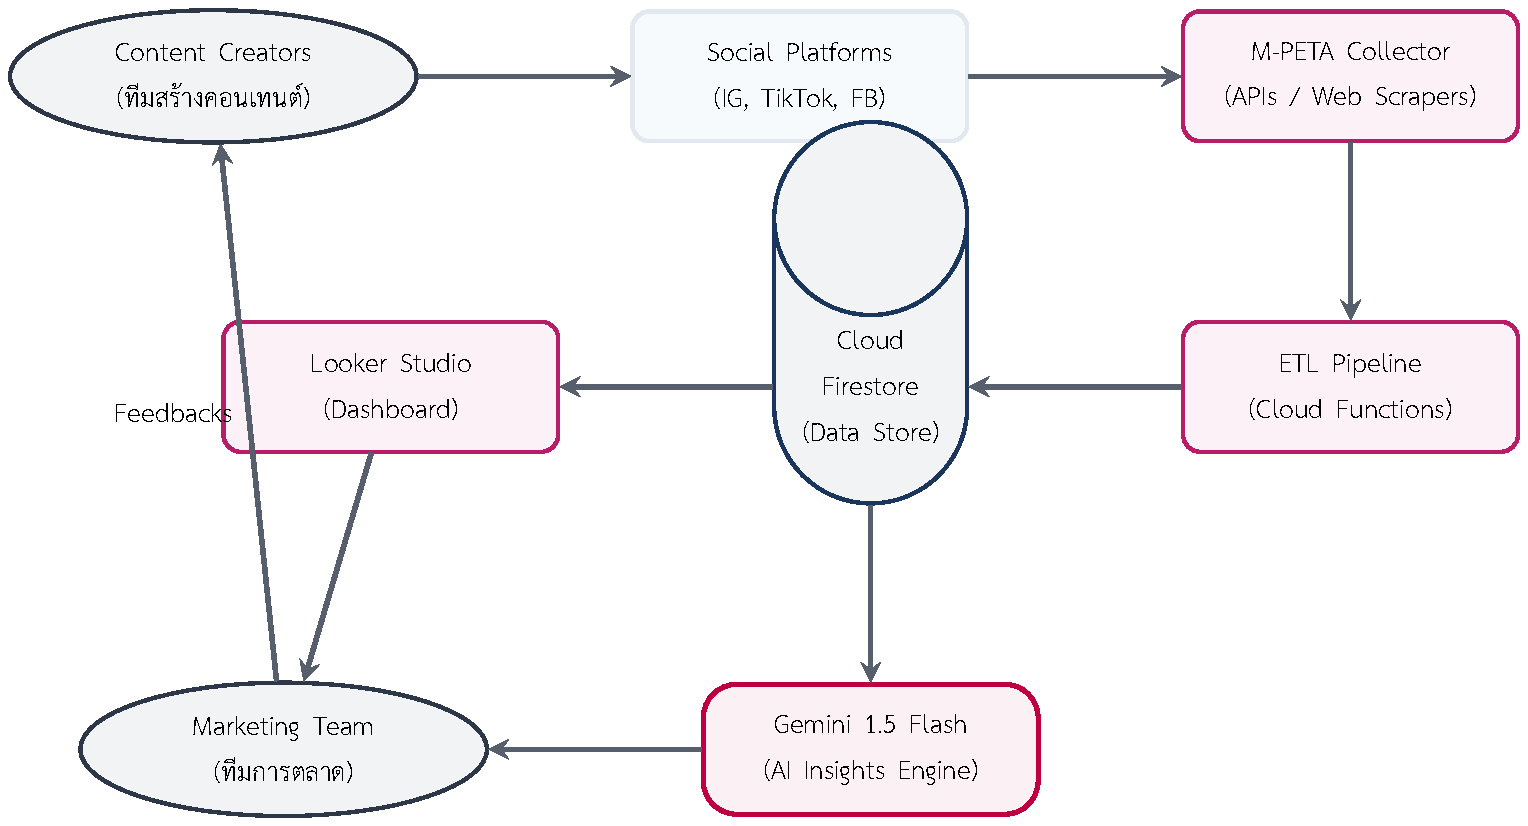
\includegraphics[width=0.75\textwidth]{diagram_marketing.png}
  \caption{\chulafont ภาพรวมระบบดึงข้อมูล 3 ช่องทางสำรองของ Social Pulse --- ระบบเลือกช่องทางจากบนลงล่างอัตโนมัติ}
\end{figure}
\vskip 0.2cm

\subsection{ขั้นที่ 2 — เก็บข้อมูล: ข้อมูลไหลจากที่ไหนไปที่ไหน?}
หลังจากดึงข้อมูลได้แล้ว ระบบเก็บข้อมูลเป็น 2 ชั้น โดยมีหน้าที่ต่างกันชัดเจน --- \textbf{ไม่ใช่ทางเลือก แต่คือขั้นตอนที่ต่อกัน}:
\begin{itemize}
  \item \textbf{ชั้นที่ 1 --- เก็บชั่วคราวใน \logobadge{Sheets}{Google Sheets} (แก้ไขได้ง่าย)}: n8n เขียนข้อมูลรายวันเข้า Sheets ก่อน เพราะสมาชิกทั่วไปเข้าถึงได้ทันที และสามารถแก้ไขข้อมูลผิดพลาดได้โดยไม่ต้องรู้เทคนิค
  \item \textbf{ชั้นที่ 2 --- ซิงก์ถาวรลง \logobadge{Supabase}{Supabase PostgreSQL} ทุกคืน (คลังหลัก)}: ข้อมูลจาก Sheets จะถูกรวมเข้าฐานข้อมูลกลาง Supabase โดยอัตโนมัติ เพื่อให้ Dashboard ดึงไปแสดงผลได้รวดเร็วและรองรับการเชื่อมข้อมูลข้ามแผนกในภายหลัง
  \item \textbf{ชั้นที่ 3 --- แสดงผลผ่าน \logobadge{PowerBI}{Power BI Desktop} (วิเคราะห์เชิงลึก)}: เชื่อมตรงกับ Supabase เพื่อให้ฝ่าย Innovation ใช้สูตร DAX วิเคราะห์เปรียบเทียบข้อมูลข้ามช่วงเวลาได้
  \item \textbf{ชั้นที่ 4 --- ถามข้อมูลด้วยภาษาคนผ่าน Claude Chat (ใช้งานง่ายที่สุด)}: สมาชิกพิมพ์ถามว่า "โพสต์เดือนนี้ ER เฉลี่ยเท่าไหร่?" ได้ตรงเลยโดยไม่ต้องเปิด Dashboard ผ่านระบบ MCP Client ที่เชื่อมกับ Supabase
\end{itemize}

\subsection{ขั้นที่ 3 — วิเคราะห์: สูตรที่ระบบคำนวณให้อัตโนมัติ}
เมื่อข้อมูลเข้า Supabase แล้ว ระบบจะคำนวณตัวชี้วัด 3 ตัวให้ทันทีโดยไม่ต้องให้ทีมมานั่งคำนวณเอง ตัวชี้วัดเหล่านี้บอกว่าคอนเทนต์ "ดีแค่ไหน" และ "กำลังจะหมดความนิยมหรือยัง":
\begin{enumerate}[label=\bfseries สูตรที่ \arabic*:]
  \item \textbf{Engagement Rate --- ER (คอนเทนต์นี้คนสนใจมากแค่ไหน?)}: วัดว่าในบรรดาคนที่เห็นโพสต์นี้ มีกี่เปอร์เซ็นต์ที่ลงมือทำอะไรบางอย่าง (ไลก์ คอมเมนต์ แชร์ หรือบันทึกไว้) งานวิจัยของ Keib et al. (2018) [2] พบว่าตัวเลข ER สำคัญกว่ายอดผู้ติดตามถึง 3.2 เท่า ในการพยากรณ์ว่าช่องนั้นจะเติบโตได้จริงในระยะยาวหรือไม่
    \begin{equation}
      ER = \left( \frac{\text{Likes} + \text{Comments} + \text{Shares} + \text{Saves}}{\text{Reach}} \right) \times 100
    \end{equation}
  \item \textbf{Virality Score --- VS (คอนเทนต์นี้คนอยากส่งต่อแค่ไหน?)}: วัดสัดส่วนคนที่แชร์ต่อออกไปเทียบกับคนที่เห็น Berger \& Milkman (2012) [1] พบว่าคอนเทนต์ที่ viral มักมี VS สูงเสมอ เพราะกระตุ้นอารมณ์แรง หรือมีประโยชน์ที่คนอยากบอกต่อ
    \begin{equation}
      VS = \left( \frac{\text{Shares}}{\text{Reach}} \right) \times 100
    \end{equation}
  \item \textbf{Content Decay Rate --- CDR (คอนเทนต์นี้ "หมดอายุ" เร็วแค่ไหน?)}: วัดว่า ER ของโพสต์ลดลงกี่เปอร์เซ็นต์ภายใน 7 วัน ใช้ตัดสินใจว่าควร boost โพสต์ต่อ หรือปล่อยให้หายไปตามธรรมชาติ
    \begin{equation}
      CDR = \left( \frac{ER_{\text{Day1}} - ER_{\text{Day7}}}{ER_{\text{Day1}}} \right) \times 100
    \end{equation}
\end{enumerate}

\subsection{ขั้นที่ 4 — แสดงผล: ตัวอย่างข้อมูลที่ระบบจัดเก็บและแสดงบน Dashboard}
ตารางด้านล่างแสดงตัวอย่างโครงสร้างข้อมูลจริงที่ระบบ Social Pulse จะเก็บไว้ใน Supabase --- สังเกตว่าแต่ละแถวมีคอลัมน์ \textbf{Data Source} บอกว่าข้อมูลแถวนั้นมาจากช่องทางไหน (API / Vision / MCP / Scraper) และมี \textbf{Campaign Tag} เชื่อมกับค่าใช้จ่ายในฝ่ายการเงินเพื่อคำนวณ ROI ได้ในภายหลัง:
\begin{table}[h!]
  \centering
  \caption{\chulafont โครงสร้างชุดข้อมูลสถิติคอนเทนต์ระบบ M-PETA v2}
  \begin{tabular}{lllrrrcll}
    \toprule
    \textbf{Post ID} & \textbf{Platform} & \textbf{Content Type} & \textbf{Reach} & \textbf{Engage} & \textbf{ER (\%)} & \textbf{VS (\%)} & \textbf{Data Source} & \textbf{Campaign Tag} \\
    \midrule
    IG\_2601 & Instagram & Reel & 4,500 & 900 & 20.0 & 4.2 & \logobadge{Meta}{API} & Recruiter-2026 \\
    TT\_2602 & TikTok & Video & 18,200 & 2,730 & 15.0 & 5.1 & \logobadge{Gemini}{Vision} & Recruiter-2026 \\
    FB\_2603 & Facebook & Image & 1,100 & 55 & 5.0 & 0.3 & \logobadge{Playwright}{MCP} & Workshop-AI \\
    TT\_2605 & TikTok & Reel & 9,500 & 1,710 & 18.0 & 4.8 & \logobadge{Apify}{Scraper} & Recruiter-2026 \\
    \bottomrule
  \end{tabular}
\end{table}

\newpage

\section{ฝ่าย Finance: ระบบแปลงใบเสร็จภาพถ่ายให้เป็นรายการบัญชีอัตโนมัติ "ClearBook"}

\noindent ปัญหาเดิมคือสมาชิกจ่ายเงินซื้อของแล้วส่งใบเสร็จในแชตส่วนตัว ซึ่งหายได้ ตกหล่นได้ และต้องมีคนมานั่งรวบรวมอีกหลายวัน ClearBook แก้ปัญหานี้ด้วยกระบวนการ 5 ขั้น ตั้งแต่สมาชิกถ่ายรูปใบเสร็จจนถึงตัวเลขปรากฏบน Dashboard ของผู้บริหาร โดยใช้เวลาน้อยกว่า 10 นาที

\subsection{ภาพรวม 5 ขั้นตอน: ใบเสร็จเดินทางอย่างไรผ่านระบบ?}
แต่ละขั้นตอนออกแบบให้ไม่ทับซ้อนกัน (MECE) และครอบคลุมทั้งกระบวนการ ตั้งแต่ต้นน้ำ (สมาชิกถ่ายรูป) จนถึงปลายน้ำ (ผู้บริหารดูรายงาน) ดังแผนภาพด้านล่าง:

\begin{figure}[h!]
  \centering
  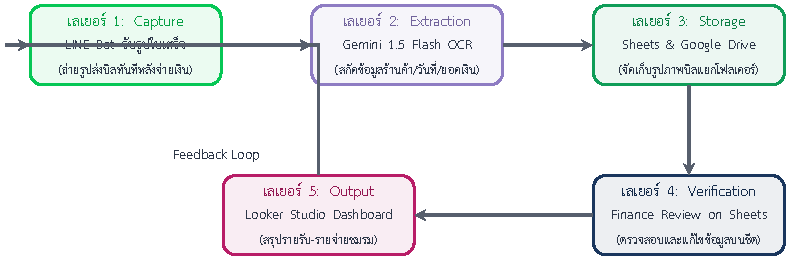
\includegraphics[width=0.95\textwidth]{diagram_mece.png}
  \caption{\chulafont ภาพรวม 5 ขั้นตอนของระบบ ClearBook --- ใบเสร็จเดินทางจากมือสมาชิกถึง Dashboard ผู้บริหาร}

โดยสามารถอธิบายแต่ละขั้นตอนได้ดังนี้ พร้อมบอกว่า \textbf{สมาชิกต้องทำอะไร} และ \textbf{ระบบทำอะไรให้อัตโนมัติ}:
\begin{itemize}
  \item \textbf{ขั้น 1 --- รับใบเสร็จ (สมาชิกทำ 10 วินาที)}: ถ่ายภาพใบเสร็จแล้วส่งเข้า \logobadge{LINE}{LINE Bot} ของชมรม ระบุชื่อแคมเปญที่ใช้จ่าย --- แค่นี้คือทุกสิ่งที่สมาชิกต้องทำ ไม่ต้องพิมพ์ตัวเลขเอง
  \item \textbf{ขั้น 2 --- อ่านตัวเลขจากภาพ (ระบบทำเอง)}: \logobadge{Gemini}{Gemini OCR} สแกนภาพใบเสร็จแล้วดึงข้อมูลออกมาเป็นโครงสร้าง JSON อัตโนมัติ ได้แก่ ร้านค้า ยอดเงิน วันที่ รายการสินค้า ไม่มีการพิมพ์ตัวเลขด้วยมือ จึงไม่มีความผิดพลาดจากคน
  \item \textbf{ขั้น 3 --- บันทึกและจัดเก็บ (ระบบทำเอง)}: ข้อมูลถูกเขียนลง \logobadge{Sheets}{Google Drive \& Sheets} และจัดแฟ้มภาพใบเสร็จตามปี เดือน และฝ่าย เพื่อให้ตรวจสอบย้อนหลังได้ทุกเมื่อ
  \item \textbf{ขั้น 4 --- ให้ผู้มีอำนาจอนุมัติ (ทีมการเงินทำ 1 คลิก)}: ระบบส่งข้อความพร้อมภาพใบเสร็จไปที่ \logobadge{Discord}{Discord Webhook} ของทีมการเงิน มีปุ่ม "อนุมัติ" และ "ปฏิเสธ" ให้กดได้ในแชตเลย และระบบแจ้งเตือนหากมีใบเสร็จซ้ำกันในคลัง
  \item \textbf{ขั้น 5 --- แสดงรายงานสรุป (ผู้บริหารดูได้เรียลไทม์)}: รายงานทางการเงินปรากฏบน \logobadge{PowerBI}{Looker Studio} ทันทีที่มีการอนุมัติ พร้อมแจ้งเตือนอัตโนมัติหากงบใกล้เต็ม
\end{itemize}

\subsection{ลำดับขั้นตอนแบบละเอียด: ใบเสร็จ 1 ใบ ผ่านระบบอย่างไร?}
\begin{enumerate}
  \item \textbf{สมาชิกส่งหลักฐาน}: ถ่ายภาพใบเสร็จ ส่งเข้า LINE Bot ของชมรม และเลือกชื่อแคมเปญที่ใช้จ่ายเงินนั้น
  \item \textbf{AI อ่านตัวเลขจากภาพ}: Gemini 1.5 Flash API สแกนและดึง ร้านค้า ยอดเงินรวม วันที่ รายการสินค้า และหมวดหมู่ออกมาเป็นข้อมูลดิจิทัล
  \item \textbf{ทีมการเงินกดอนุมัติในแชต}: ระบบส่งสรุปคู่รูปใบเสร็จไปที่ Discord ทีมการเงินกด "อนุมัติ" หรือ "ปฏิเสธ" ได้เลย --- และระบบจะแจ้งเตือนทันทีหากใบเสร็จนั้นซ้ำกับรายการที่เคยบันทึกไว้แล้ว
  \item \textbf{จัดเก็บและสรุปบัญชีอัตโนมัติ}: ไฟล์ถูกเปลี่ยนชื่อตามรูปแบบมาตรฐานและย้ายเข้าคลัง ตัวเลขถูกบันทึกลงชีตและ Supabase พร้อมอัปเดต Dashboard ทันที
\end{enumerate}

\vskip 0.2cm
\begin{figure}[h!]
  \centering
  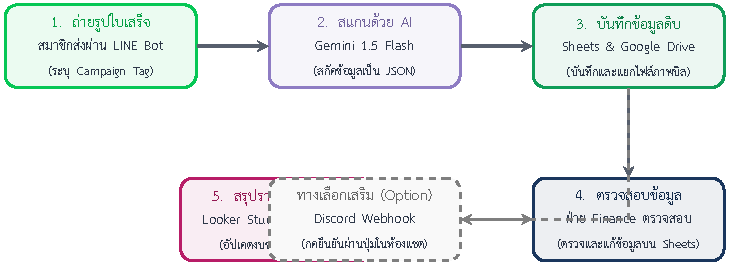
\includegraphics[width=0.75\textwidth]{diagram_finance.png}
  \caption{\chulafont สถาปัตยกรรมกระบวนการตรวจสอบเอกสารและเบิกจ่ายเงินของระบบ ClearBook}
\end{figure}
\vskip 0.2cm

\subsection{ตัวอย่างข้อมูลที่ระบบบันทึก: ตารางรายการเบิกจ่าย ClearBook}
สังเกตว่าทุกแถวมีคอลัมน์ \textbf{Campaign Tag} ซึ่งเป็นตัวเชื่อมกับยอด Reach ในตาราง Social Pulse --- ทำให้ระบบสามารถคำนวณ CPR / CPE ของแต่ละแคมเปญได้อัตโนมัติ:
\begin{table}[h!]
  \centering
  \caption{\chulafont ตัวอย่างตารางรายการเบิกจ่ายระบบ ClearBook}
  \begin{tabular}{lllrccl}
    \toprule
    \textbf{TX ID} & \textbf{Submitter} & \textbf{Dept} & \textbf{Amount} & \textbf{Store Name} & \textbf{Status} & \textbf{Campaign Tag} \\
    \midrule
    TX-2601 & Four & Innovation & 450.00 & Cafe Amazon & Approved & Recruiter-2026 \\
    TX-2602 & Peach & Marketing & 1,500.00 & Meta Ads & Approved & Recruiter-2026 \\
    TX-2603 & Guy & Activity & 3,200.00 & Somtum Shop & Pending & Workshop-AI \\
    \bottomrule
  \end{tabular}
\end{table}

\newpage

\section{จุดรวมของทั้งสองระบบ: Campaign Tag เชื่อม Marketing กับ Finance เพื่อวัด ROI}
\subsection{Campaign Tag คืออะไร และทำให้ระบบฉลาดขึ้นอย่างไร?}
ทั้ง Social Pulse และ ClearBook ทำงานได้ดีอยู่แล้วแยกกัน แต่จุดที่ระบบ Club OS แตกต่างจากเครื่องมือทั่วไปคือการที่ทั้งสองโมดูลใช้รหัสเชื่อมกัน --- \textbf{Campaign Tag} --- เพื่อให้ฝ่ายบริหารตอบคำถามสำคัญที่สุดได้: \emph{"เราใช้เงินไปเท่าไหร่ แล้วได้ผลกลับมาแค่ไหน?"}

\begin{highlightbox}
  \noindent \textbf{กลไกการเชื่อมข้อมูลข้ามแผนก}

  เมื่อสมาชิกยิงโฆษณาและส่งใบเสร็จเข้า ClearBook โดยระบุ Campaign Tag ว่า "Recruiter-2026" ในเวลาเดียวกัน Social Pulse ก็ดึงสถิติของโพสต์ที่ใช้ Campaign Tag เดียวกันนั้น ระบบหลังบ้านใน Supabase จะ \textbf{จับคู่ทั้งสองตารางเข้าหากันโดยอัตโนมัติ} และแสดงผลบน Looker Studio ว่าแคมเปญนั้นคุ้มค่าแค่ไหน โดยไม่ต้องให้ใครมานั่งรวมข้อมูลด้วยมือเลย ซึ่งสอดคล้องกับกรอบแนวคิดของ Chaffey \& Ellis-Chadwick (2019) [3] ที่ระบุว่าการวัดประสิทธิภาพสื่อดิจิทัลที่แม่นยำต้องเชื่อมงบประมาณจริงเข้ากับพฤติกรรมผู้ชม เพื่อหลีกเลี่ยงการตัดสินใจจากตัวเลข "ยอดผู้เข้าถึง" เปล่า ๆ ที่ไม่บอกความคุ้มค่าที่แท้จริง
\end{highlightbox}

\begin{equation}
  \text{Cost per Reach (CPR)} = \frac{\text{ยอดเงินใช้จ่ายรวมในโครงการ (จาก ClearBook)}}{\text{ยอดจำนวนการเข้าถึงรวม (จาก Social Pulse)}}
\end{equation}
\begin{equation}
  \text{Cost per Engagement (CPE)} = \frac{\text{ยอดเงินใช้จ่ายรวมในโครงการ (จาก ClearBook)}}{\text{ยอดจำนวนการมีส่วนร่วมรวม (จาก Social Pulse)}}
\end{equation}

\vskip 0.2cm
\begin{figure}[h!]
  \centering
  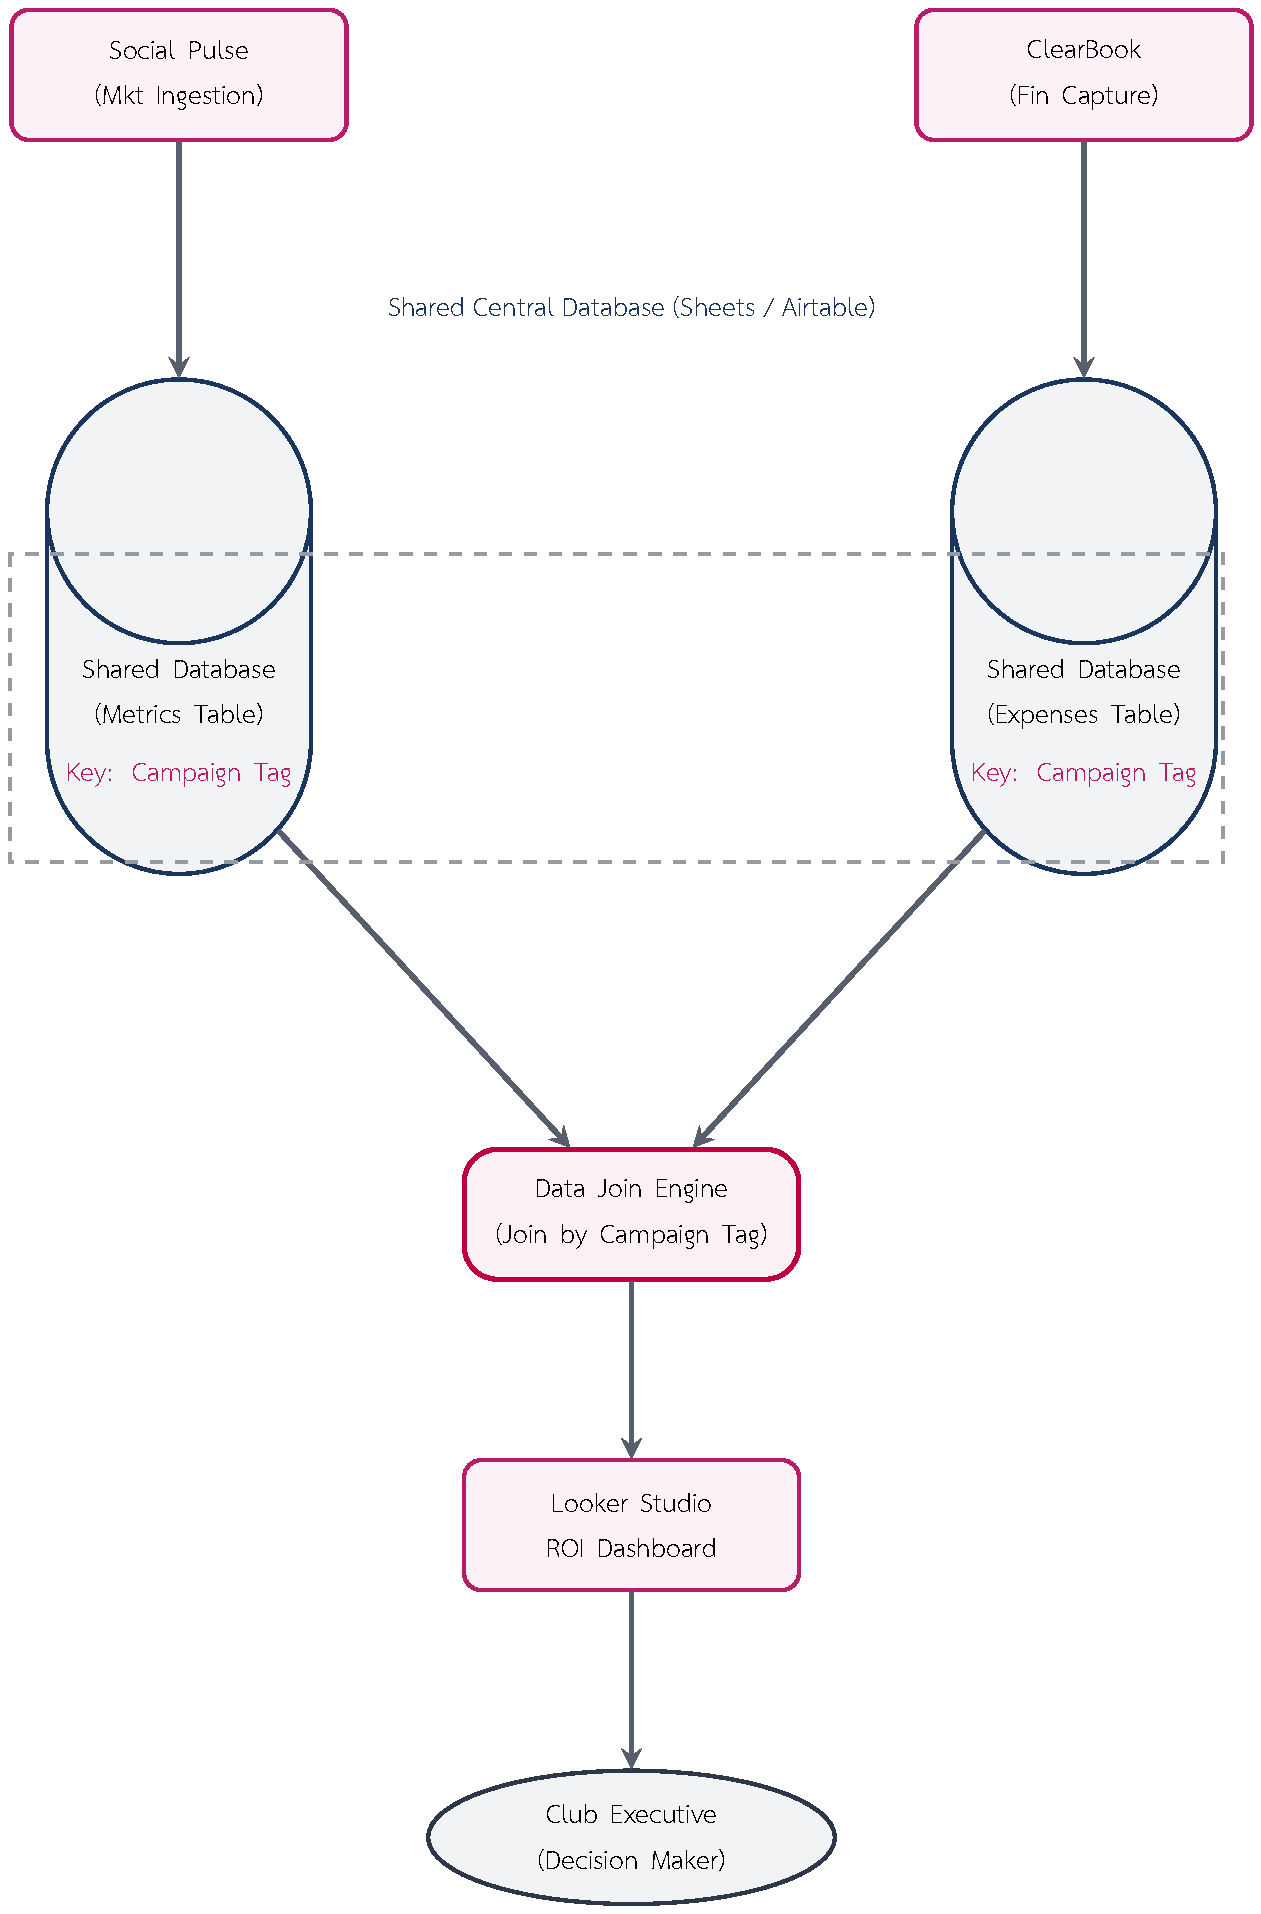
\includegraphics[width=0.75\textwidth]{diagram_club_os.png}
  \caption{\chulafont แผนภาพการเชื่อมโยงระบบข้อมูลข้ามแผนกเพื่อประเมินประสิทธิภาพแคมเปญร่วมกัน}
\end{figure}
\vskip 0.2cm

\subsection{ตัวเลขจริงพิสูจน์ว่าใช้ได้: 2 แคมเปญตัวอย่างที่ระบบวิเคราะห์ได้ทันที}
\begin{itemize}
  \item \textbf{แคมเปญรับสมัครสมาชิกใหม่ (Recruiter-2026)}: ยอดรายจ่ายยิงโฆษณาและค่าโปสเตอร์รวม 1,950 บาท (\logobadge{LINE}{ClearBook}) แลกกับสถิติการดึงดูดยอดผู้เห็นรวม 22,700 Reach และมีส่วนร่วม 3,630 Engage (\logobadge{Meta}{Social Pulse}) คิดเป็น \textbf{CPR 0.08 บาทต่อ Reach} และ \textbf{CPE 0.53 บาทต่อ Engagement}
  \item \textbf{แคมเปญกิจกรรมสัมมนา (Workshop-AI)}: ยอดรายจ่ายรวม 3,200 บาท แลกกับยอดผู้เข้าถึงต่ำเนื่องจากโพสต์แค่รูปเดี่ยว ส่งผลให้ CPR/CPE สูงผิดปกติ ฝ่ายบริหารวิเคราะห์จุดนี้และสั่งปรับเปลี่ยนรูปแบบการโปรโมตเวิร์กชอปครั้งหน้าไปเป็นวิดีโอสั้นทันที
\end{itemize}

\newpage

\section{ทำไมถึงเลือกเครื่องมือชุดนี้? เหตุผลและบทบาทของแต่ละตัว}
\subsection{ตารางสรุปเครื่องมือทั้งหมดในระบบ Club OS พร้อมเหตุผล}
เครื่องมือทุกตัวถูกเลือกโดยมีเกณฑ์ 3 ข้อ คือ \textbf{ฟรีหรือต้นทุนต่ำ} (ชมรมไม่มีงบซอฟต์แวร์), \textbf{สมาชิกทั่วไปใช้ได้ไม่ต้องมีความรู้เทคนิค} และ \textbf{เชื่อมต่อกับเครื่องมืออื่นในระบบได้} ดังแสดงในตารางด้านล่าง:

\begin{table}[h!]
  \centering
  \caption{\chulafont ตารางวิเคราะห์เครื่องมือเทคโนโลยีและเหตุผลการเลือกใช้ในระบบ Club OS}
  \begin{tabular}{llp{4.5cm}p{7.0cm}}
    \toprule
    \textbf{ระบบย่อย} & \textbf{เครื่องมือ} & \textbf{บทบาทหน้าที่} & \textbf{เหตุผลและขีดความสามารถที่คัดเลือก} \\
    \midrule
    Marketing & \logobadge{n8n}{n8n} & Workflow Orchestration & รองรับการรันลูปดึงข้อมูลรายวันแบบไม่เสียค่าใช้จ่ายผ่าน Free Tier และทำระบบสลับช่องทางสำรอง (Fallback) ได้สะดวก \\
    & \logobadge{Playwright}{Playwright} & Web automation (Fallback) & เข้าถึงข้อมูลหลังบ้านหน้าเว็บได้แม้ยอด API จะชน Rate Limit หรือช่องทาง API ปกติขัดข้อง \\
    & \logobadge{Apify}{Apify} & Public web scraping & สกัดข้อมูลสาธารณะจากหน้าร้านภายนอกโดยไม่ต้องยืนยันตัวตน \\
    \midrule
    Finance & \logobadge{LINE}{LINE Bot} & User Interface (Input) & สมาชิกทุกคนคุ้นเคยเป็นอย่างดี ถ่ายภาพและกรอกชื่อแคมเปญส่งได้ทันทีใน 10 วินาที \\
    & \logobadge{Gemini}{Gemini Flash} & OCR \& Structured Extraction & สกัดข้อมูลตัวเลข ร้านค้า วันที่ รายการสินค้า จากภาพใบเสร็จออกมาเป็น JSON ได้ถูกต้องรวดเร็วด้วยราคาที่ประหยัดที่สุด \\
    & \logobadge{Discord}{Discord Webhook} & Approval Channel & ระบบส่งการแจ้งเตือนและมีปุ่มอนุมัติสำหรับฝ่ายการเงินภายในเครื่องมือสื่อสารที่ใช้เป็นปกติ \\
    \midrule
    Club OS & \logobadge{Supabase}{Supabase DB} & Core Storage Layer & ฐานข้อมูล PostgreSQL สำหรับการเก็บข้อมูลถาวร รองรับการเชื่อมโยงตารางข้อมูลข้ามแผนก และรวบรวมเพื่อทำ Analytics \\
    & \logobadge{Sheets}{Google Sheets} & Operational Spreadsheet & บันทึกข้อมูลสำรองที่แก้ไขง่าย เหมาะสำหรับสมาชิกที่ไม่มีความรู้เชิงเทคนิคในการแก้ไขเบื้องต้น \\
    & \logobadge{PowerBI}{Looker / Power BI} & Visualization Dashboard & ประมวลผลและแสดงรายงานดัชนีชี้วัด CPR/CPE และงบประมาณคงเหลือแบบเรียลไทม์ \\
    \bottomrule
  \end{tabular}
\end{table}

\subsection{ผลลัพธ์ที่คาดหวังหลังใช้ระบบ: ตัวเลขเปรียบเทียบก่อนและหลัง}
Club OS ไม่ได้แค่ "สะดวกขึ้น" แต่ตัดงานซ้ำซากออกไปแทบทั้งหมด และยกระดับคุณภาพการตัดสินใจของทีมบริหารในสองด้าน:
\begin{enumerate}
  \item \textbf{ด้านการตลาด --- ทีมได้กลับมาโฟกัสงานสร้างสรรค์:} ปัจจุบันสมาชิกฝ่ายการตลาดต้องใช้เวลา 3--4 ชั่วโมงต่อสัปดาห์ในการนั่งรวบรวมตัวเลขจากหลายแพลตฟอร์มมาใส่ตาราง เมื่อระบบ Social Pulse ดึงข้อมูลให้อัตโนมัติทุกคืน เวลานั้นจะเหลือ 0 นาที ทีมสามารถหันไปโฟกัสงาน creative และทดลองแคมเปญใหม่ได้แทน ซึ่งสอดคล้องกับงานวิจัยของ Järvinen \& Karjaluoto (2015) [4] ที่พบว่าระบบ analytics อัตโนมัติช่วยให้ทีมทดลองและปรับแคมเปญได้รวดเร็วและคุ้มค่ากว่าอย่างมีนัยสำคัญ
  \item \textbf{ด้านการเงิน --- จาก 3--5 วัน เหลือ 10 นาที:} กระบวนการบันทึกและตรวจสอบใบเสร็จที่ปัจจุบันใช้เวลา 3--5 วันทำการ จะเหลือเพียง 5--10 นาทีหลังทำธุรกรรม และเนื่องจาก AI อ่านตัวเลขจากภาพโดยตรง จึงไม่มีความเสี่ยงจากการพิมพ์ตัวเลขผิด งานวิจัยของ Willcocks, Lacity, \& Craig (2015) [5] และ Lacity \& Willcocks (2016) [6] ยืนยันว่าการนำ Robotic Process Automation มาใช้กับงานเอกสารซ้ำซาก สามารถลดเวลาธุรกรรมได้ถึง 75--90\% พร้อมกับเพิ่มความถูกต้องของข้อมูลทางบัญชีได้อย่างสมบูรณ์แบบ
\end{enumerate}

\newpage

\section{แผนพัฒนาและตัวชี้วัด: สร้างและทดสอบระบบภายใน 5 สัปดาห์}
\subsection{ลำดับการพัฒนา: สร้างอะไรก่อน สร้างอะไรทีหลัง?}
ระบบถูกแบ่งเป็น 3 ช่วงโดยเรียงลำดับความสำคัญจาก "ให้สมาชิกใช้ได้จริงก่อน" แล้วค่อยเพิ่ม automation และการเชื่อมข้ามแผนกในภายหลัง:
\begin{table}[h!]
  \centering
  \caption{\chulafont แผนกำหนดการพัฒนาระบบย่อย Club OS}
  \begin{tabular}{llp{11.0cm}}
    \toprule
    \textbf{ระยะเวลา} & \textbf{เป้าหมาย (Phase)} & \textbf{กิจกรรมและการดำเนินงานหลัก} \\
    \midrule
    \textbf{สัปดาห์ที่ 1--2} & MVP Core Launch & พัฒนา LINE Bot สแกนใบเสร็จด้วย Gemini 1.5 Flash (Finance) และแบบฟอร์มบันทึกการตลาดสำรอง \\
    \textbf{สัปดาห์ที่ 3--4} & Full Automation & พัฒนา n8n workflow ดึงข้อมูล API อัตโนมัติรายวัน และระบบ verify ผ่านปุ่ม Discord/LINE \\
    \textbf{สัปดาห์ที่ 5} & Club OS Integration & เชื่อมตารางข้อมูลข้ามฝ่ายผ่าน Campaign Tag และทำสรุปแดชบอร์ด Campaign ROI ใน Looker Studio \\
    \bottomrule
  \end{tabular}
\end{table}

\subsection{สรุปก่อนและหลัง: ระบบ Club OS เปลี่ยนแปลงอะไรบ้างในการทำงานของชมรม?}
\begin{table}[h!]
  \centering
  \caption{\chulafont เปรียบเทียบประสิทธิภาพก่อนและหลังปรับปรุงระบบ}
  \begin{tabular}{lll}
    \toprule
    \textbf{ตัวชี้วัดที่ทำการประเมิน} & \textbf{ระบบเดิม (Manual Process)} & \textbf{ระบบใหม่แบบอัตโนมัติ (Club OS)} \\
    \midrule
    \textbf{ระยะเวลาจัดเก็บสถิติ Marketing} & 3-4 ชั่วโมง ต่อสัปดาห์ (พิมพ์มือ) & 0 นาที (n8n ดึงข้อมูลเบื้องหลังอัตโนมัติ) \\
    \textbf{เวลาเฉลี่ยบันทึก/ตรวจสอบใบเสร็จ} & 3-5 วันทำการ (เอกสารกระจัดกระจาย) & 5-10 นาที (สแกน OCR ทันทีที่จ่ายเงิน) \\
    \textbf{ความถูกต้องของหลักฐานการเบิกจ่าย} & ปานกลาง (มีความเสี่ยงยอดพิมพ์ผิด) & 100\% (ผ่านการสกัดจากภาพและมีระบบตรวจสอบสองชั้น) \\
    \textbf{การเข้าถึงข้อมูลเพื่อตัดสินใจเชิงรุก} & ล่าช้า และข้อมูลไม่เกิดการเชื่อมกัน & รายงานดัชนี CPR/CPE ข้ามแผนกแบบเรียลไทม์ \\
    \textbf{งบประมาณซอฟต์แวร์ของชมรม} & 0 บาท (ใช้แรงงานซ้ำซาก) & 0 บาท (ใช้งาน Cloud Free Tiers และ Open-source) \\
    \bottomrule
  \end{tabular}
\end{table}

\subsection{เอกสารอ้างอิงงานวิจัยที่ใช้สนับสนุนการออกแบบระบบ}
\begin{enumerate}[label={[\arabic*]}]
  \item Berger, J., \& Milkman, K. L. (2012). What Makes Online Content Viral? \textit{Journal of Marketing Research}, 49(2), 192--205. https://doi.org/10.1509/jmr.10.0353
  \item Keib, K., Himelboim, I., \& Han, J. Y. (2018). Important tweets matter: Predicting retweets in the \#BlackLivesMatter talk on Twitter. \textit{Computers in Human Behavior}, 85, 106--115. https://doi.org/10.1016/j.chb.2018.03.025
  \item Chaffey, D., \& Ellis-Chadwick, F. (2019). \textit{Digital Marketing: Strategy, Implementation and Practice} (7th ed.). Pearson.
  \item Järvinen, J., \& Karjaluoto, H. (2015). The use of Web analytics for digital marketing performance measurement. \textit{Industrial Marketing Management}, 50, 117--127. https://doi.org/10.1016/j.indmarman.2015.04.009
  \item Willcocks, L., Lacity, M., \& Craig, A. (2015). Robotic Process Automation at Xchanging. \textit{The Outsourcing Unit Working Research Paper Series}, Paper 15/03.
  \item Lacity, M., \& Willcocks, L. (2016). Robotic Process Automation and Cognitive Technology: The Next Frontier. \textit{SB Publishing}.
\end{enumerate}

\end{document}
